
%%%%%%%%%%%%%%%%%%%%%%%%%%%%%%%%%%%%%%%%%%%%%%%%%%%%%%%%%%%%%%%%%%%%
\chapter{Review of epidemiological behavioural and opinion models in literature}
\label{ch:literature_review}
%NUOVO TESTO
The scientific community's interest in epi-behavior models has existed for several years. Initially, as noted by \cite{Bauch_2012_overview}, the behavioral aspect of epidemiology was not given significant attention. Its development has been a gradual process, resulting from years of evolution in research.

In fact, in the epidemiological initial works, the focus of scientists was primarily on presenting the evolution of diseases. The resulting models did not account for the effect of behavior; the population was considered homogeneously mixed, leading to random contact between susceptibles and infectious \cite{Hernandez_Vargas_2022, Mata2021}. 
It was only later, as epidemiological models proved effective and reliable in describing and predicting disease spread, that interest in their beneficial impact on population safety and well-being grew. Tools that integrate real data with epidemiological models emerged, helping inform decisions on matters such as school closures or travel restrictions, as described in \cite{Bauch_2012_overview}.

Furthermore, new categories of models have emerged, such as agent-based models, networked models, and multi-layer/multi-system models. Despite their differing approaches, they aim to integrate various population characteristics, for example contact structure, age distribution, and movement patterns, to address the limitations of the original homogeneity assumption \cite{brauer2012mathematical}.
This focus on societal composition and behavior naturally stems from the desire to use modeling tools as a reference for decision-making in safety and health. 

One possible approach is to incorporate changes in the structure of models that describe aspects of behavior or population composition. In these models, the behavior of the population is implicitly considered by integrating time-variable parameters that capture changes in societal behavior. This approach represents the classical modeling technique used in the formulation of epidemiological models. Examples of studies that uses this methodology for analyzing COVID-19 include \cite{Giordano_2020, Dehning_2020, Proverbio_2021}.

Although models developed in this way have proven to be powerful tools for generating insights about disease dynamics and providing recommendations to policymakers, they fall short in their ability to accurately reconstruct how populations behave during an epidemic outbreak. The desire to explore this aspect and develop a framework capable of simultaneously simulating both behavior and disease diffusion—where each mutually influences the other—has driven the development of a specific research field dedicated to behavioral epidemics.

But how can behavior be integrated into pre-existing epidemiological theory? To better address this question, we follow the classification proposed in \cite{Funk_2010}, which offers a possible subdivision of behavioral literature based on the different approaches that most articles focus on. Three major categories emerge:
\begin{itemize}
	\item The source of information used to make decisions;
	\item The type of information used to make decisions;
	\item The effect of behavioral change on the dynamic described by  the model. 
\end{itemize}


The first two points focus on distinguishing between the various strategies implemented to model and integrate information dynamics, which play a crucial role in behavioral models. In this context, information acts as the infectious agent within the social layer. Models incorporate this effect in different ways, highlighting how messages are communicated—whether through media or conversation—and the type of information researchers choose to emphasize (e.g., fear of the disease or data on infection numbers). The last categorization is dedicated to the different strategies used to integrate human behavior into these models.
\section{Information's sources}
When analyzing the source of information, there is a clear distinction between works \cite{Vogiatzis2010} that assume governments and populations base their decisions on precise data, such as the number of infected individuals (prevalence) \cite{Collinson2014, Tyson_2020}, and those that consider more informal sources, such as conversations between people, public opinion, or media \cite{Bulai2023, Sontag2022}. These media sources include both traditional outlets like television and newspapers, as well as newer platforms like social networks.
This distinction highlights the diversity in how behavioral factors are integrated into models, reflecting the varying degrees of reliability and influence these sources have on decision-making processes during an epidemic.


Regarding information quality and the negative effect of misinformation spreading within the population, an example is the fear of vaccination \cite{Kahan_2013}. Several works analyze its effects to on the spread of infection \cite{Bauch_2012_game, Epstein_2021}.
An example of how this phenomenon can occur is the case of an article originally published by a prestigious source. Although the thesis presented in this work, which claimed a correlation between the measles, mumps, and rubella (MMR) vaccine and autism or other gastrointestinal disorders, was later debunked by the scientific community and the article retracted \cite{wakefield1998retracted}, the negative impact in terms of spreading fear about vaccines has persisted. In many cases, this fear has become deeply ingrained, leading to a reduction in herd immunity and a resurgence of measles \cite{Bauch_2012_overview}.

\section{Classification of different types of information}
After introducing the impact that the quality of information can have, another interesting aspect relates to the different types of information used as a basis for developing a new model. Choosing a specific type of information leads to the creation of distinct models that focus on different aspects of behavior. Some studies focus on the influence of media on behavior \cite{Collinson2014, Misra_2011}, while others examine peer-to-peer conversations, information exchange, and individual beliefs \cite{Tyson_2020}. These are completely different approaches, even though they aim to achieve the same effect: simulating the evolution of people's opinions and behavior. Using media involves hypothesizing that the population is influenced by a few "central" information nodes, so the same news, data, or future predictions are shared with everyone. In contrast, models that use personal information exchanges can depict a scenario where many different ideas about the disease situation circulate simultaneously.
Another concept used in models that simulate a sort of "collective consciousness" is referred to as "awareness" \cite{Funk2009}. To model how awareness spreads in the population, it is often treated like a disease \cite{Silva2019, Granell2013, Granell_2014, Kabir_2019, Zuo_2021, Wang_2019}. Although there are many differences between these two, the main idea is that theories and concepts about a certain topic can spread among people, which can be considered at a higher level as a unified opinion. For example, there may be many different personal positions on how to respond to a health emergency like COVID-19, but it is possible to abstract the various opinions and reconstruct what the majority of people, or macro-groups, ultimately feel. They may either be more cooperative and in favor of following guidelines issued by authorities, or more focused on their well-being and inclined to act independently.
This process can be related to opinion formation studies, which aim to understand how people build their ideas \cite{Devia_2023, Devia2022} and also analyze the possible formation of opinion distributions, such as perfect consensus, consensus, polarization, clustering, or dissension.

\section{How to integrate behavior in epidemiology}
While the type and source of information are crucial for understanding the basic framework and synthesizing key concepts of models that consider population behavior, the final criterion used to categorize works related to epidemiological behavior is how the influence of people's behavior on the model is integrated. This aspect is one of the most interesting and was a key focus of the literature reviewed for this thesis, as it plays a significant role in comparing and selecting relevant works for this research.

There are various ways to describe behavior in response to an epidemic and integrate this aspect into epidemic models \cite{Wang_2019, Bedson2021, Wang_2015_review}.

The first approach involves observing and simulating how connected individuals' states are linked to specific behaviors and how this influences the epidemic. This category includes agent-based models. Additionally, the reverse relationship, where disease spread alters individual behavior, has also been considered, as discussed in \cite{Granell_2014}.

There is also a broad class of mean-field models that explicitly consider the effects of behavior. In these cases, time-varying or state-varying parameters are used, resulting in a non-linear system of equations where the parameters are not constant but change based on information such as disease prevalence. Refer to paragraph \ref{subsec:homogeneous} for further details on this topic.

Another possibility involves modifying the structure or connections in the network used to simulate disease evolution \cite{Peng2021}. In network-based models, data extracted from social network structures \cite{Carballosa_2021} or small-world models \cite{Turker_2023} are often used to simulate connections between people more realistically.

In the following paragraphs, several articles are presented using this classification to simplify their categorization. Each article is then discussed in more detail, highlighting its original contribution.

\subsection{Individuals-based models}
\label{subsec:individual_state}
\subsubsection{Multiple networks simulated with Markovian process}
To begin the presentation of individual-based models, the first category discussed is network simulations using Markovian processes. A notable example is the article by Granell et al. \cite{Granell_2014}. In this work, a multiplex model is implemented with two distinct connectivity layers: the physical layer, where the disease spreads, and the virtual contact layer, through which "awareness" about the disease diffuses. Awareness is in the knowledge about how reduce the risk of infection, and diffuses through conversation or is due to becoming infected. The article then uses the Microscopic Markov Chain approach to simulate the interaction resulting from the coupling of the two layers. Interestingly, they observe the existence of a metacritical point for the onset of the epidemic, which depends on awareness dynamic and topology of the virtual network. There is, in fact, a parameter related to the ability to influence through communication and it is observed that it impacts the onset of the epidemic only when it exceeds a certain threshold.
A subsequent work of the same authors \cite{Granell2013}, considers also the effect of a global communication agent. In this case, the metacritical point disappears. 
\begin{figure}[h]
	\centering
	\subfloat[][\emph{}]
	{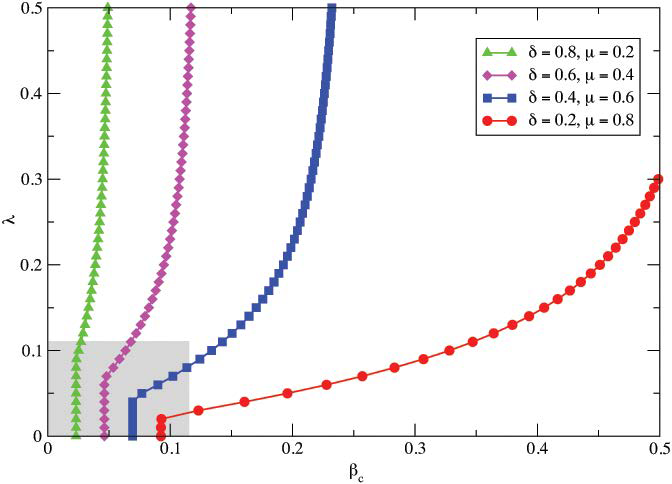
\includegraphics[width=0.47\linewidth]{0_introduction/images_review/metacritical_point_granell_2013}} \quad
	\subfloat[][\emph{}]
	{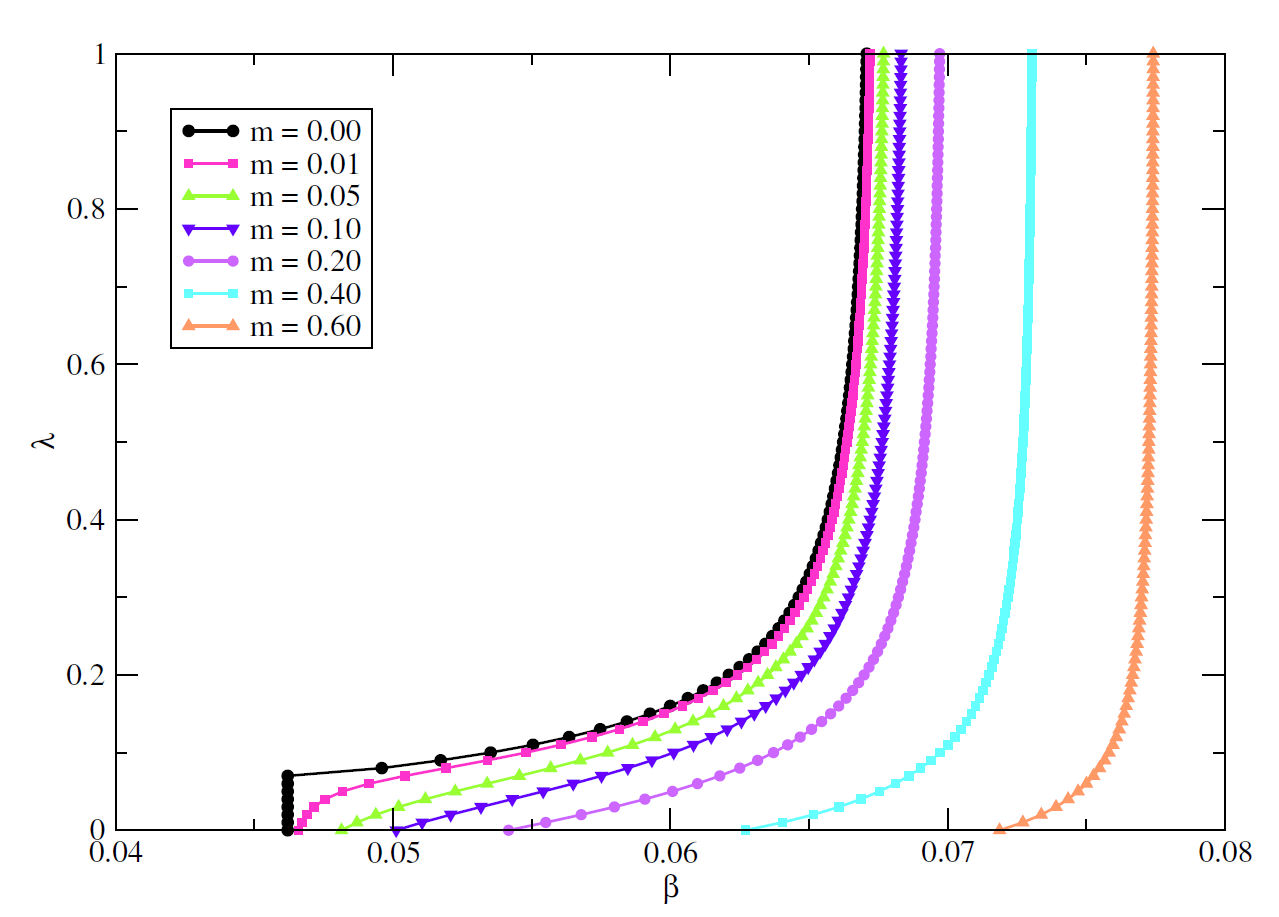
\includegraphics[width=0.49\linewidth]{0_introduction/images_review/metacritical_point_granell_2014}} \\
	\caption[Metacritical effect]{The effect of awareness communication on the onset of an epidemic is depicted in the studies by Granell et al. \cite{Granell2013, Granell_2014}. In the first plot (a), the x-axis represents the minimum value of the transmission rate $\beta$ that is necessary to trigger an outbreak, while the y-axis measures the level of awareness in the population, denoted by the parameter $\lambda$. The shaded region shows that below a critical threshold of $\lambda$, awareness has little to no impact on controlling the epidemic. However, once awareness exceeds this threshold, the value of $\beta$ required for an outbreak increases significantly, indicating that the spread of awareness can effectively delay or prevent the epidemic. In contrast, in the second plot (b), a global communication agent, represented by the media parameter $m$, continuously influences the population. This parameter ensures that the awareness layer consistently impacts the epidemic dynamics, regardless of the value of $\lambda$, making it evident that a strong media presence can amplify the protective effects of awareness.}
	\label{fig:sir_example2}
\end{figure}


In the article by \cite{Sahneh2013}, there is a complete description of the stochastic process at the agent level, which is useful for understanding how agent interactions are modeled across different layers using a Markovian approach. Other works using this method include \cite{Silva2019, Frieswijk_2022, Peng2021, Zuo_2021}. Except for \cite{Frieswijk_2022}, a similar double-layer structure, composed of an SIR model coupled with an unaware-aware-unaware (UAU) process, is presented in the other articles. To simulate the evolution of the complex structure resulting from the coupling of the two models, they build transition trees for all possible state changes and their respective transition probabilities. An example of both can be seen in figure \ref{fig:sir_example3}.  

\begin{figure}[h]
	\centering
	\subfloat[][\emph{}]
	{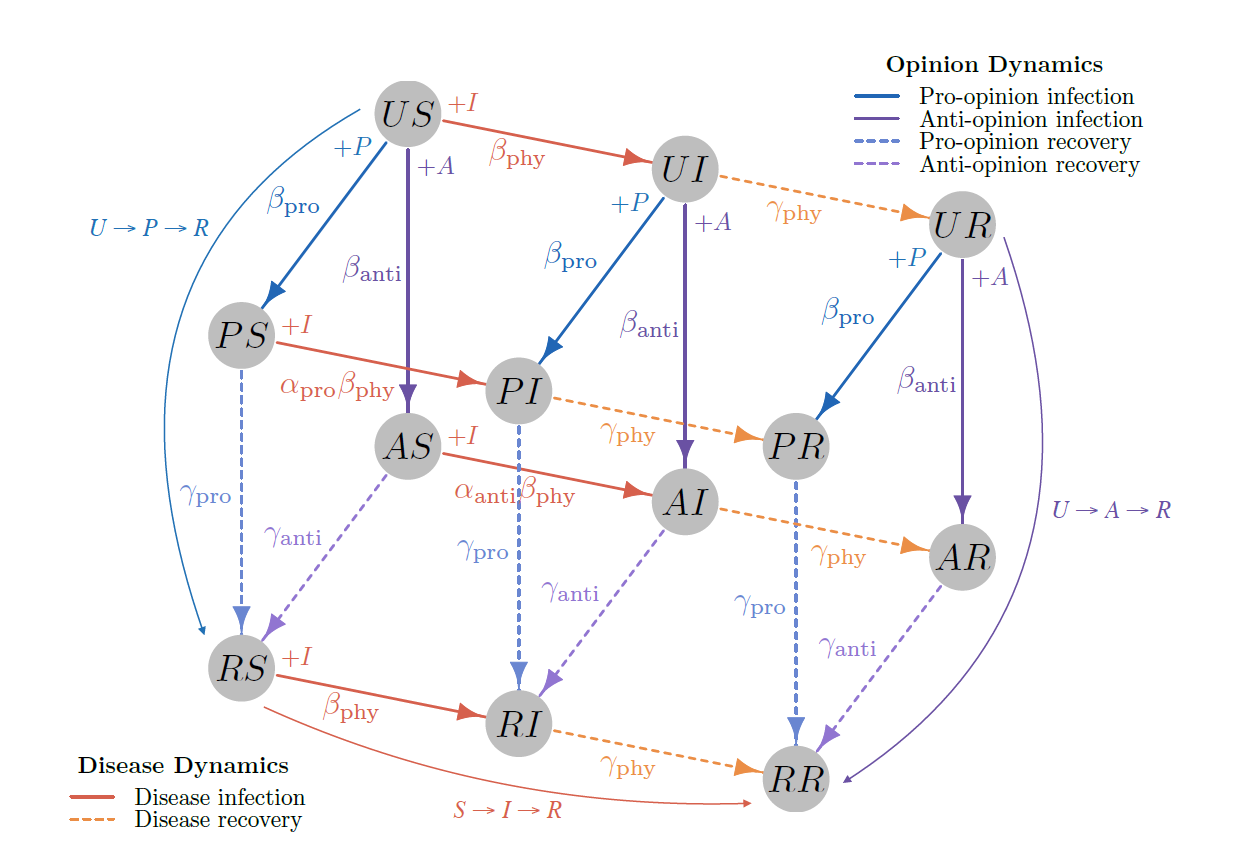
\includegraphics[width=0.63\linewidth]{0_introduction/images_review/peng_2021_bertozzi_coupled_structure}} \quad
	\subfloat[][\emph{}]
	{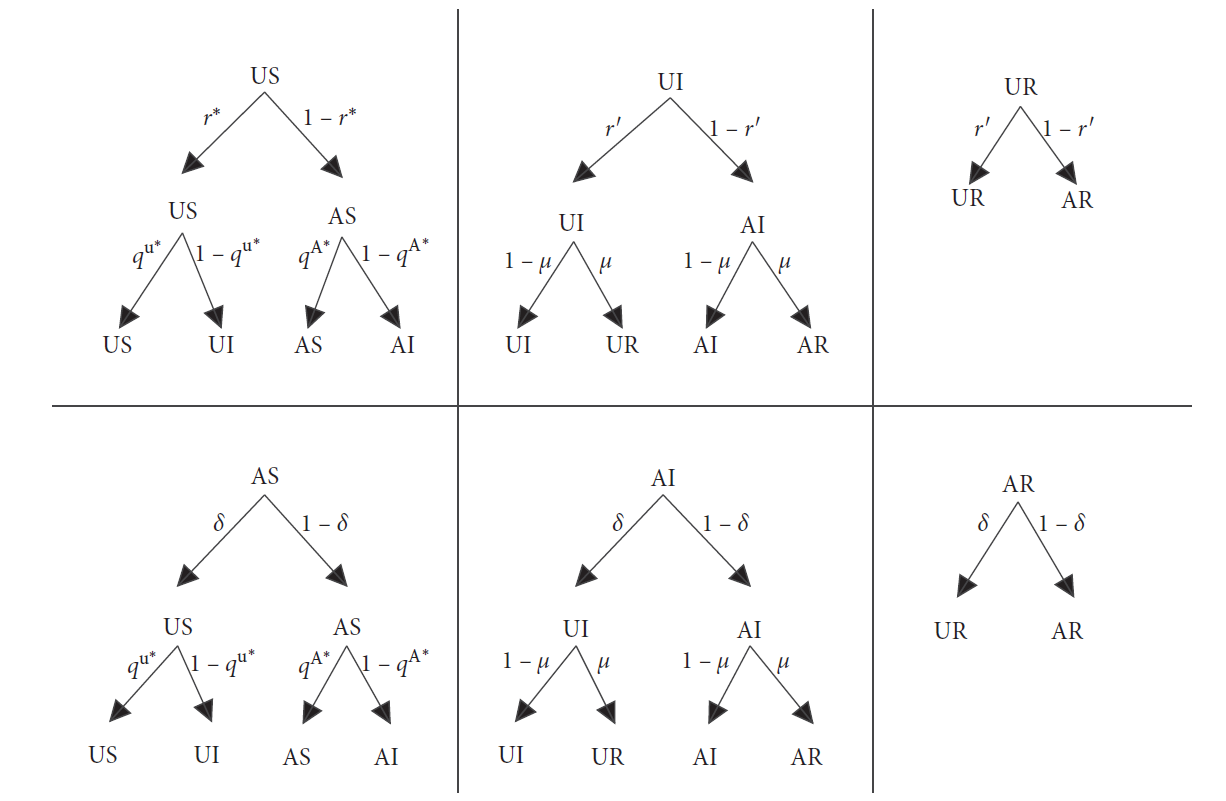
\includegraphics[width=0.6\linewidth]{0_introduction/images_review/silva2019_transition_trees}} \\
	\caption[Multiplex networks]{a) An example of a multiplex network structure resulting from the coupling of a SIR and a uninformed-pro/anti physical distance-recovered (U-P/A-R) model. b) The transition trees realized to describe the system of a SIR coupled  with a UAU model using a Markovian process. Pictures taken from articles \cite{Peng2021, Silva2019}.}
	\label{fig:sir_example3}
\end{figure}

In \cite{Peng2021}, a slightly more complex situation is described, where two possible opinions—pro-physical distancing (P) and anti-physical distancing (A)—are considered. In contrast, \cite{Frieswijk_2022} studies a simpler structure, where a SIS model is coupled with either adopting or not adopting self-protective measures.

Interesting results derived from these works include: 
\begin{itemize} 
	\item The observation of the influence of opinions on transmission speed and the final epidemic size \cite{Peng2021}. 
	\item The effect on epidemic spreading of authoritative information, publicizing epidemic prevention processes, and encouraging reasonable behavior, such as isolating when infected \cite{Zuo_2021}. 
	\item The importance of self-awareness as a mechanism to reduce disease prevalence \cite{Silva2019}. 
\end{itemize}

The simulations conducted in \cite{Frieswijk_2022} provide a stability analysis of a two-layer model that links the decision to use or not use self-protection measures with the disease state. The equilibria of the system are explicitly calculated, including the epidemic threshold. Figure \ref{fig:stability_friesjiw} illustrates their simulations, where a parameter representing risk perception is varied. The study shows how this parameter influences the emergence of periodic oscillations and identifies the conditions that lead to global convergence towards such periodic solutions. This is a significant result, indicating that during an epidemic, there is a collective behavioral response, and it specifies under what conditions the system stabilizes or becomes dynamic.

\begin{figure}[h]
	\centering
	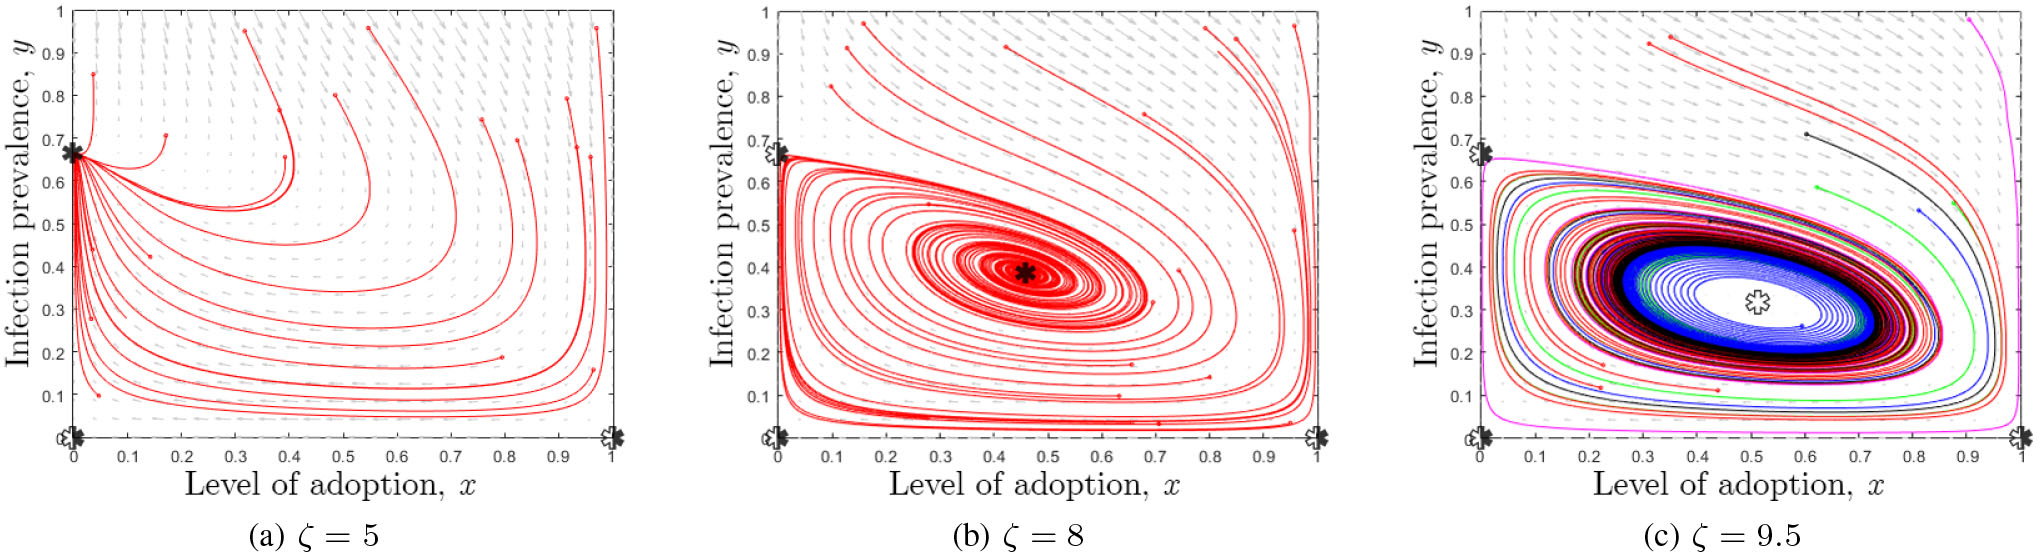
\includegraphics[width=0.95\linewidth]{0_introduction/images_review/stable_unstable_equilibria_friejs}
	\caption[Stability analysis of epi-behavior model]{Simulations from the article \cite{Frieswijk_2022} demonstrate the evolution of their model across various values of the risk perception parameter. In the visual representation, the x-axis shows the adoption level of precautionary measures, while the y-axis indicates the prevalence reached by the infection. The diagram highlights stable equilibria, saddle points, and unstable equilibria, which are marked with black, black-white, and white asterisks, respectively.}
	\label{fig:stability_friesjiw}
\end{figure}

\subsubsection{Game theoretical models}
In the probabilistic framework, another area involves the use of game theory principles. These are used to explore strategic interactions between individuals, where participants act to maximize their utility, potentially influencing the actions of others. The concept of Nash Equilibrium is also important in this context. It is defined as "a set of strategies such that no player has an incentive to unilaterally deviate from the present strategy" \cite{Wang_2015_review}. That is, the Nash Equilibrium leads individuals to adopt strategies consistent with their goal of maximizing their benefit or utility in a perfectly rational way, forming the best responses to one another.

Many articles use this idea to model how populations adjust their behavior during an epidemic. One such example is  \cite{Auld_2003}, which focuses on the behavior of a population deciding between their sexual habits and the risk of HIV infection. The main result is derived by observing how population behavior changes as information about a possible vaccine spreads. Optimistic news lead to a decrease in the number of contacts, while pessimistic forecasts cause an increase in risky behavior, even at the same level of risk, as shown in figure \ref{fig:abm_game}. A particularly interesting conclusion is that focusing public health messaging on dire forecasts may unintentionally lead to an increase in risky behavior.

\begin{figure}[h]
	\centering
	\subfloat[][\emph{}]
	{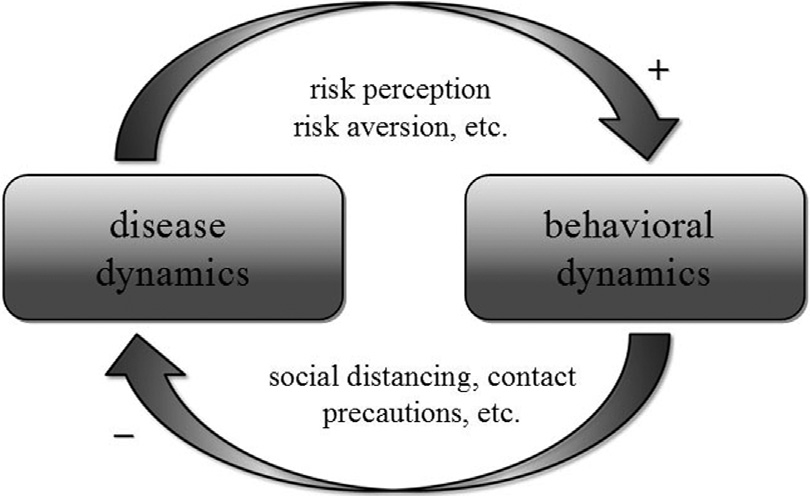
\includegraphics[width=0.38\linewidth]{0_introduction/images_review/disease_behavior_interaction_wang2015}} \quad
	\subfloat[][\emph{}]
	{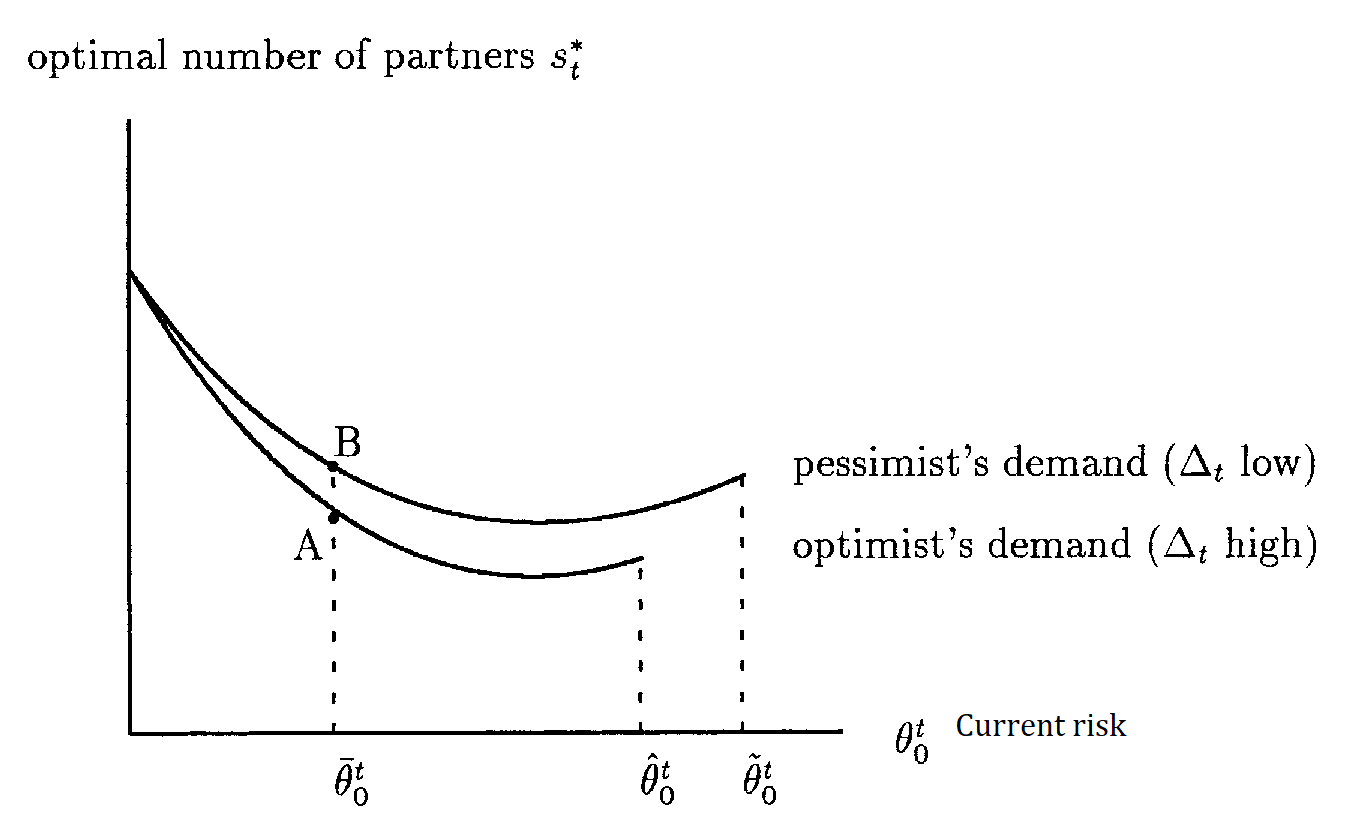
\includegraphics[width=0.58\linewidth]{0_introduction/images_review/risk_forecast_auld}} \\
	\caption[Game theory]{a) A representation of the feedback loop, taken from the article of \cite{Wang_2015}, representing the trade-off between: advantages related to avoid the disease and social cost of behave using precautions.  b) The effect on people's behavior due to optimistic or pessimistic forecasts is described in the illustration presented in \cite{Auld_2003}. The population tends to act more cautiously if there is hope that the situation will improve in the future.}
	\label{fig:abm_game}
\end{figure}

A different focus is the one that the article  \cite{Gosak_2021_game} has. Here, the behavioral change related to contact rate and especially social distancing, in the context of a pandemic situation like COVID-19  is studied to understand the efficacy of policies for partial or full voluntarily contact reduction. They aim to realize more insight into the percentage of adoption from the population of social distancing policies because increasing the quality of these estimations matters in the planning of strategies to handle a pandemic from a government point of view.

Another case study is \cite{Nunner2021}, which defines different utility functions to model the trade-off between social well-being from maintaining connections, the fatigue of doing so, and the potential physical harm those connections may cause. The main results outlined in \cite{Nunner2021} confirm that a higher number of connections between individuals leads to greater disease transmission, resulting in more infections and a shorter epidemic duration. It also highlights that "the higher the (perceived) risks of a disease, the lower the net benefit of a tie, the stronger the social distancing, and consequently the smaller the epidemic size."
Using this co-evolutionary approach, a highly correlated dynamic between the two layers emerges: a feedback loop between the spread of infection and behavioral adaptation, with structural modifications in the network occurring in the simulated scenarios.
The introduction of network-based modeling further develops this work and leads to several key findings. First, including the benefit of social connection creates multiple transmission routes for the disease. Second, a reduction in the final epidemic size only occurs when the indirect benefits are relatively low and the costs of maintaining ties are high. Finally, small changes in social behavior can have large impacts on the epidemic.
In the next paragraph, other similar studies that incorporate network models will be discussed. However, before that, a final case where the game-theoretical approach is often applied will be presented: vaccination. Many models examine the decision-making process behind vaccination, highlighting the trade-off between the benefits of getting vaccinated and the risks associated with it.
In terms of modeling, the link between behavior and epidemic spread in this case is that individuals who choose vaccination are removed from the susceptible group, with a percentage reflecting the vaccine's efficacy, thereby reducing the potential for disease transmission. In the study developed in \cite{Bauch_2012_game}, a feedback loop is established between disease prevalence and individual strategic vaccination behavior. Their model successfully fits vaccine coverage data from both the pertussis and MMR vaccine scares and can also predict future trends in disease prevalence and vaccine coverage. 
Moreover, the article highlights the phenomenon for which the vaccine fear becomes more frequent as eradication goals for more vaccine-preventable diseases are approached.

\subsubsection{Network based models}
The inclusion of networks in the modeling process has gained popularity as a tool for scientists to enhance the accuracy of their models by simulating real-world connections between people. The main goal behind developing network-based models is to create a representation of society and then use it to simulate the spread of disease. A comprehensive example of this approach is presented in \cite{VanMieghem2009}, where a method is introduced to simulate scenarios such as quarantine or regional barriers that limit population movement. By adjusting network connections—reducing contacts between nodes or cutting ties between specific regions—these models effectively demonstrate the impact of interventions like lockdowns or travel restrictions on disease transmission. They also enable analysis of how containment measures affect the trajectory of an epidemic.
Works such as \cite{Tizzoni2014} also fall into this category, utilizing urban mobility patterns as a proxy for modeling epidemics. Similarly, in \cite{Carballosa_2021}, social networks are used as a proxy for connections, hypothesizing that people's behavior in maintaining social contacts is analogous to how they might behave in the context of disease transmission.
Another innovative approach involves the development of multilayer networks, such as in \cite{Turker_2023}, where the social structure of a town is recreated. Each layer represents a different environment—ranging from homes to workplaces, distinguishing between various job types, and even considering a layer for friendships. Each individual exists across multiple layers and interacts with different groups depending on their social environment. This model found that the layer associated with friendship poses the highest risk for outbreak development, due to closer interactions and lower security measures.Consequently, even on the friendship layer, a lower transmission rate ($\beta$) compared to other layers can result in a significant epidemic involving many susceptible individuals.
\begin{figure}[h]
	\centering
	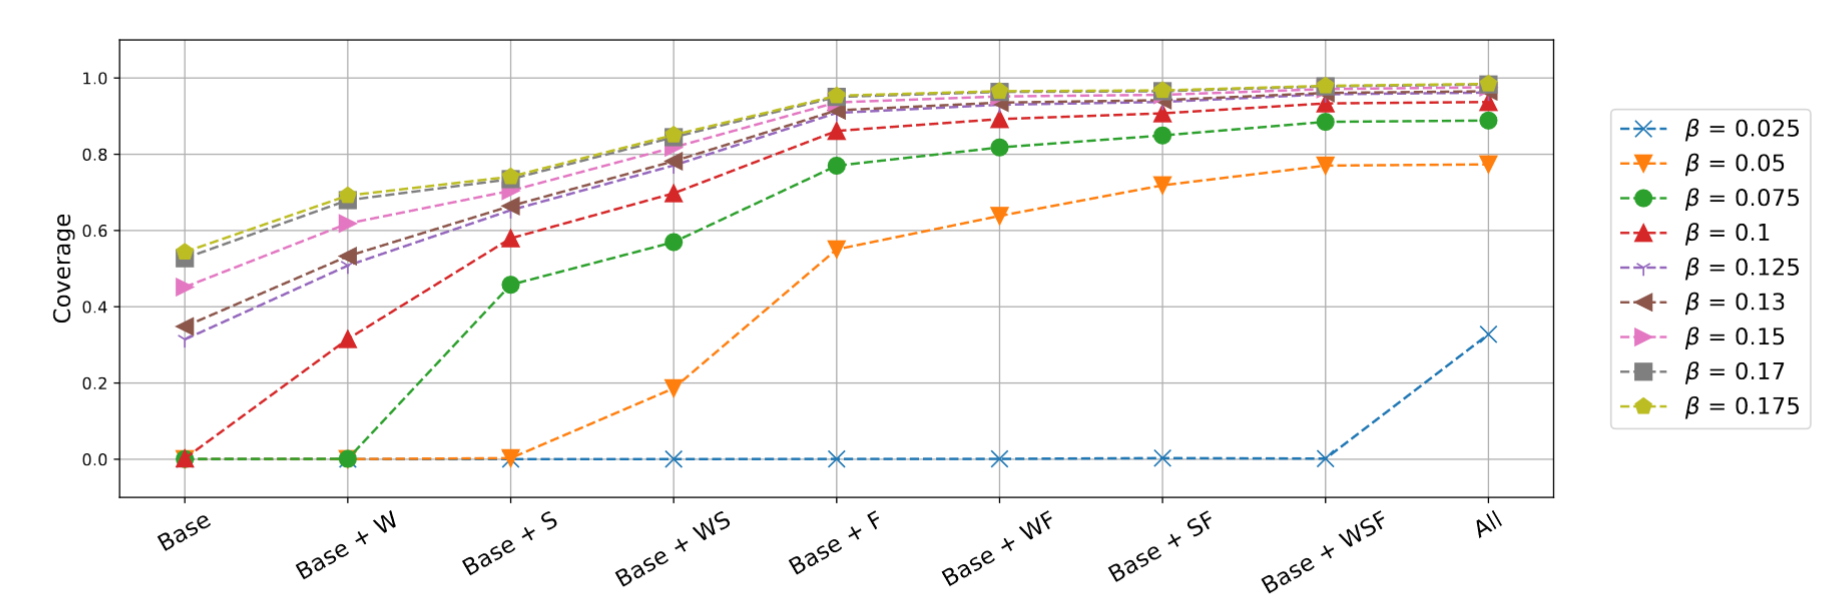
\includegraphics[width=0.9\linewidth]{0_introduction/images_review/turker_city_recreated}
	\caption[Simulation of disease spreading within a city]{In the simulation presented in \cite{Turker_2023}, a city is modeled with people divided into several social groups. They found that the layer associated with friendships is where the disease outbreak occurs with the lowest value of the infectivity parameter, $\beta$.}
	\label{fig:turkercityrecreated}
\end{figure}



\subsubsection{Threshold models}
Another possible mechanism for modeling how individuals change their actions is by observing the behaviors and opinions of their neighbors \cite{Granovetter_1978, Krassa_1988}. A well-known theoretical tool for this context is the Watts threshold model \cite{Watts_2002}, which is foundational for studying such transitions.
In \cite{Wang_2019}, various threshold models are discussed, including the Watts threshold, which is linear. In their model, each node is assigned a random threshold value based on a given distribution. The threshold represents the point at which a node changes its opinion when a certain number of its neighbors adopt a different behavior. The structure of the network is crucial for determining how opinions spread. They found that opinion propagation is most favorable in networks with low randomness and a regular structure. Additionally, they analyzed the effects of network clusters, noting that well-connected clusters can act as opinion hubs, reinforcing the spread of opinions.

\subsubsection{Ad-hoc rule-based models}
The last category of individual-based models focuses on individuals acting according to specific rules designed to simulate particular situations. A clear example of this is found in \cite{Alvarez_Zuzek_2017}, where disease propagation is modeled based on opinions for or against vaccination. The evolution of these opinions is determined by the interaction and exchange of ideas between agents and co-evolves alongside their health condition. A comprehensive set of rules is established to model all possible situations that lead to changes in both opinion and disease states. An example is visible in picture \ref{fig:alvarez_opi_vac}


\begin{figure}[h]
	\centering
	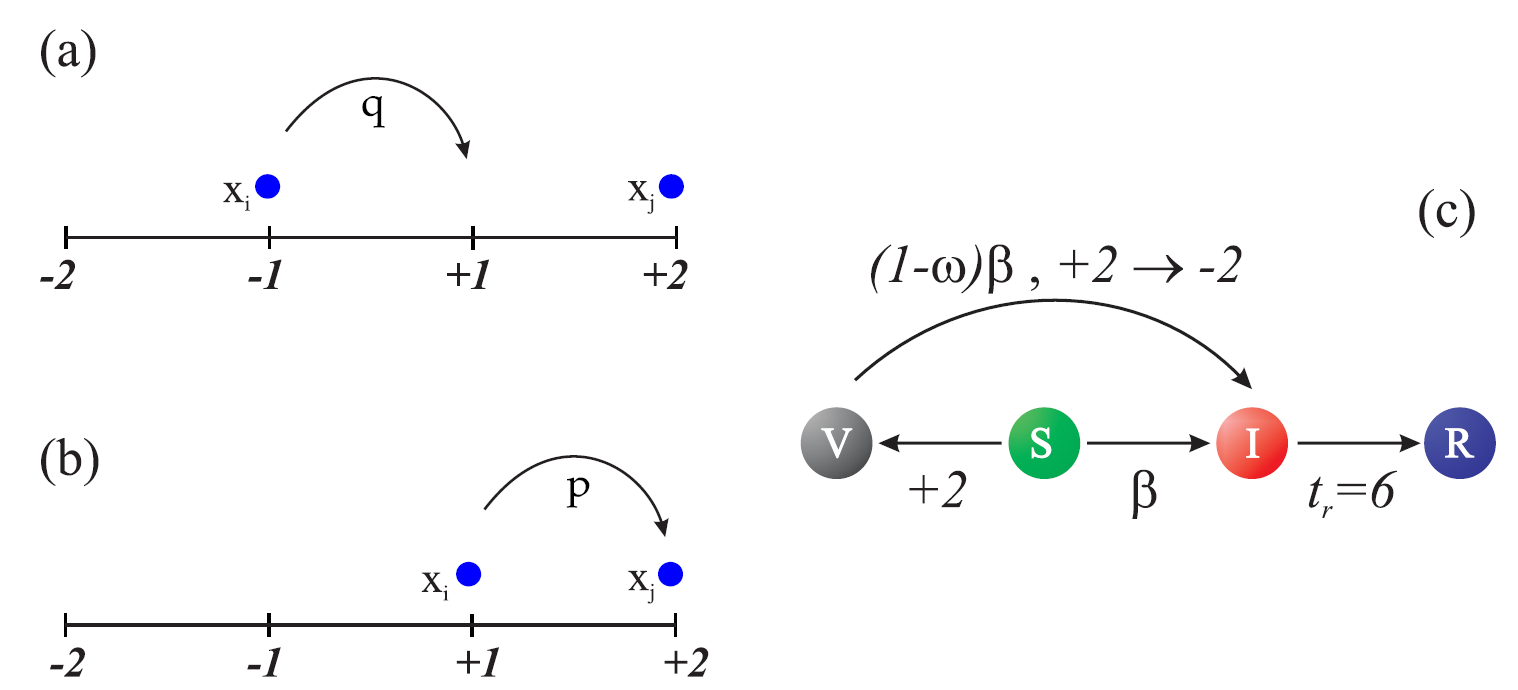
\includegraphics[width=0.8\linewidth]{0_introduction/images_review/alvarez_opi_vac}
	\caption[Rules in opinion disease model]{The picture, taken from the article \cite{Alvarez_Zuzek_2017}, illustrates the mechanisms underlying the model's dynamics. The figures on the left depict opinion dynamics: when two nodes have opposing opinions, one adjusts its state to match the other's opinion with a probability $q(a)$. If both nodes share the same opinion, the opinion is reinforced with a probability $p(b)$. The figure on the right represents contagion dynamics: a susceptible individual $S$ (green) becomes infected (red) with a probability $\beta$ and recovers (blue) after a time $t_r$. A susceptible individual can also become vaccinated $V$ (grey) upon acquiring an opinion state of $+2$. However, they can still become infected with a probability $(1-\omega) \beta$- with $\omega$ the efficiency of the vaccine- which causes their opinion to shift to $-2$. }
	\label{fig:alvarez_opi_vac}
\end{figure}

A similar approach is developed in the article by \cite{teslya2022}, where an explicit mechanism is implemented to govern the competition between different health opinions. Individuals with a positive $+$ opinion may switch to the opposing $-$ opinion after interacting with others, following a switch rate function. By varying the parameters of this function, its behavior can become linear, saturating, or sigmoidal similar to established functions used to describe predator responses to prey population density.

Finally, the article by \cite{Collinson2014} extends the SEIR model by incorporating the effect of mass media on disease spread, using a specific set of functions. These functions account for disease prevalence, recovery rate, and media impact. The goal is to conduct a sensitivity analysis on the parameters influencing the epidemic's peak magnitude, timing, and ending. 


\subsection{Homogeneous population models}
\label{subsec:homogeneous}
This section presents the works that have most contributed to shaping the development of the thesis, the mean-field models. The assumption that the population is homogeneously mixed results in models capable of describing phenomena nationwide, which is difficult to achieve when modeling individual behavior.

However, the effectiveness of this class of models relies heavily on the modeling principles applied. Models are powerful tools, but they represent the aspects the modeler chooses to emphasize. Therefore, selecting and integrating the most promising features is crucial for creating a useful instrument. By analyzing prior works, we gain insights into what has been previously explored and the outcomes achieved.
The most interesting characteristics of various models are now presented, followed by an explanation of how they have contributed to the development of the model in this thesis.

The article \cite{Tyson_2020} was one of the first studied for its insteresting modeling approach. It integrates two dynamics: the epidemic evolution influences the parameters governing people's behavior, and, conversely, the population's behavior affects the spread of the disease. This bidirectional interaction allows for a more realistic simulation of how behavioral changes and disease dynamics influence each other.
A SIR model is associated with an opinion dynamic that occurs only within the $S$ compartment. This compartment is divided into four subgroups, representing different attitudes toward prophylactic behavior. In this way, more cautious individuals have a lower probability of becoming infected. The opinion dynamic focuses on the phenomenon of influence, modeled by a specific parameter, and on opinion amplification, a cognitive bias where confronting someone with the same belief strengthens that belief.
The most interesting aspect of their work is the concept that opinion spreads through conversation, not through a utilitarian or contagion process like fear diffusion.

A similar hypothesis of social learning is explored in the article \cite{Tanaka_2002}. In this model, both risky and cautious behaviors coexist in the population and can be transmitted. The model also incorporates the effects of clustering and the phenomenon of "cultural bias." This bias suggests that the risky trait is more likely to be adopted by cautious individuals than the reverse. Additionally, the authors introduce the concept of uncertainty regarding the infection causes, meaning that people are unsure of the best way to behave to avoid contracting the disease.


In the article \cite{Bongarti2023}, compliance with the use of NPIs (Non-Pharmaceutical Interventions) is the central focus of the behavioral component of the model. In this case, non-compliance is modeled as a social contagion: the population is divided into two groups, compliant ($c$) and non-compliant ($nc$). Using the mass-action mixing property, compliant individuals become non-compliant, but there is no recovery once their status changes. The primary goal is to understand the interplay between the stringency of lockdown measures, non-compliant behavior, and the spread of the disease.


Vaccine adoption and awareness diffusion are the main arguments developed in \cite{Zuo2022}. Awareness is present only in the Susceptible compartment, and there is a term, $M(t)$, that represents the accumulated density of awareness programs driven by various information sources. This term is influenced by several factors: awareness generated by neighboring individuals, the intensity of awareness programs in response to the prevalence of the disease, and a waning effect due to the decreasing quality or effectiveness of the information over time. Their complete model and the interplay between disease and behavior is shown in figure  \ref{fig:mean_models_1}. 
An interesting aspect of this article is that the authors evaluate their model using data from the COVID-19 vaccination campaign in China. They observe how their model effectively reproduces the population behavior and government policies during different phases of the epidemic.

\begin{figure}[h]
	\centering
	\subfloat[][\emph{}]
	{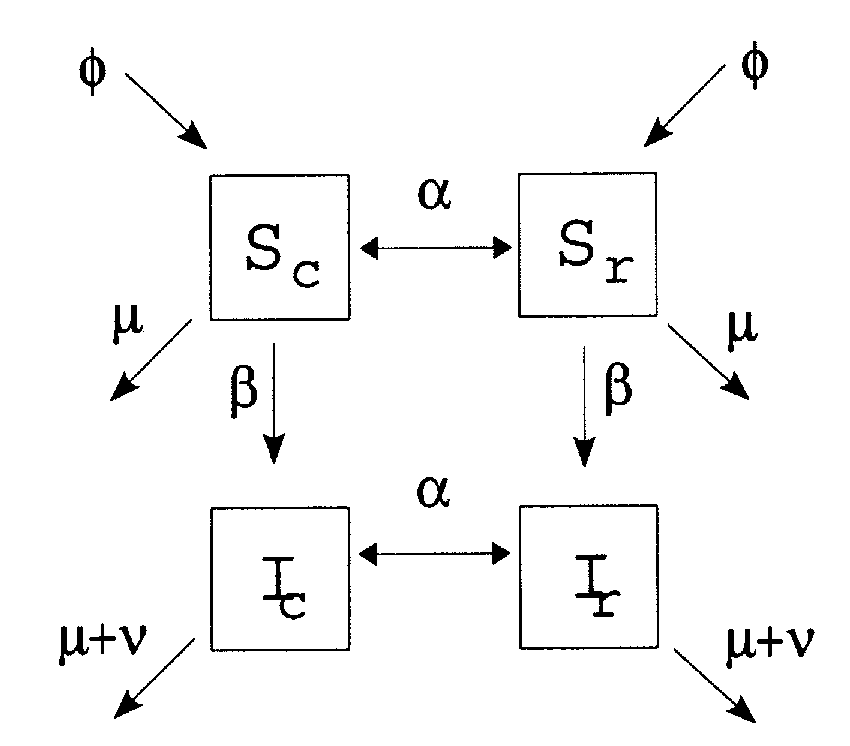
\includegraphics[width=0.35\linewidth]{0_introduction/images_review/Tanaka_model}} \quad
	\subfloat[][\emph{}]
	{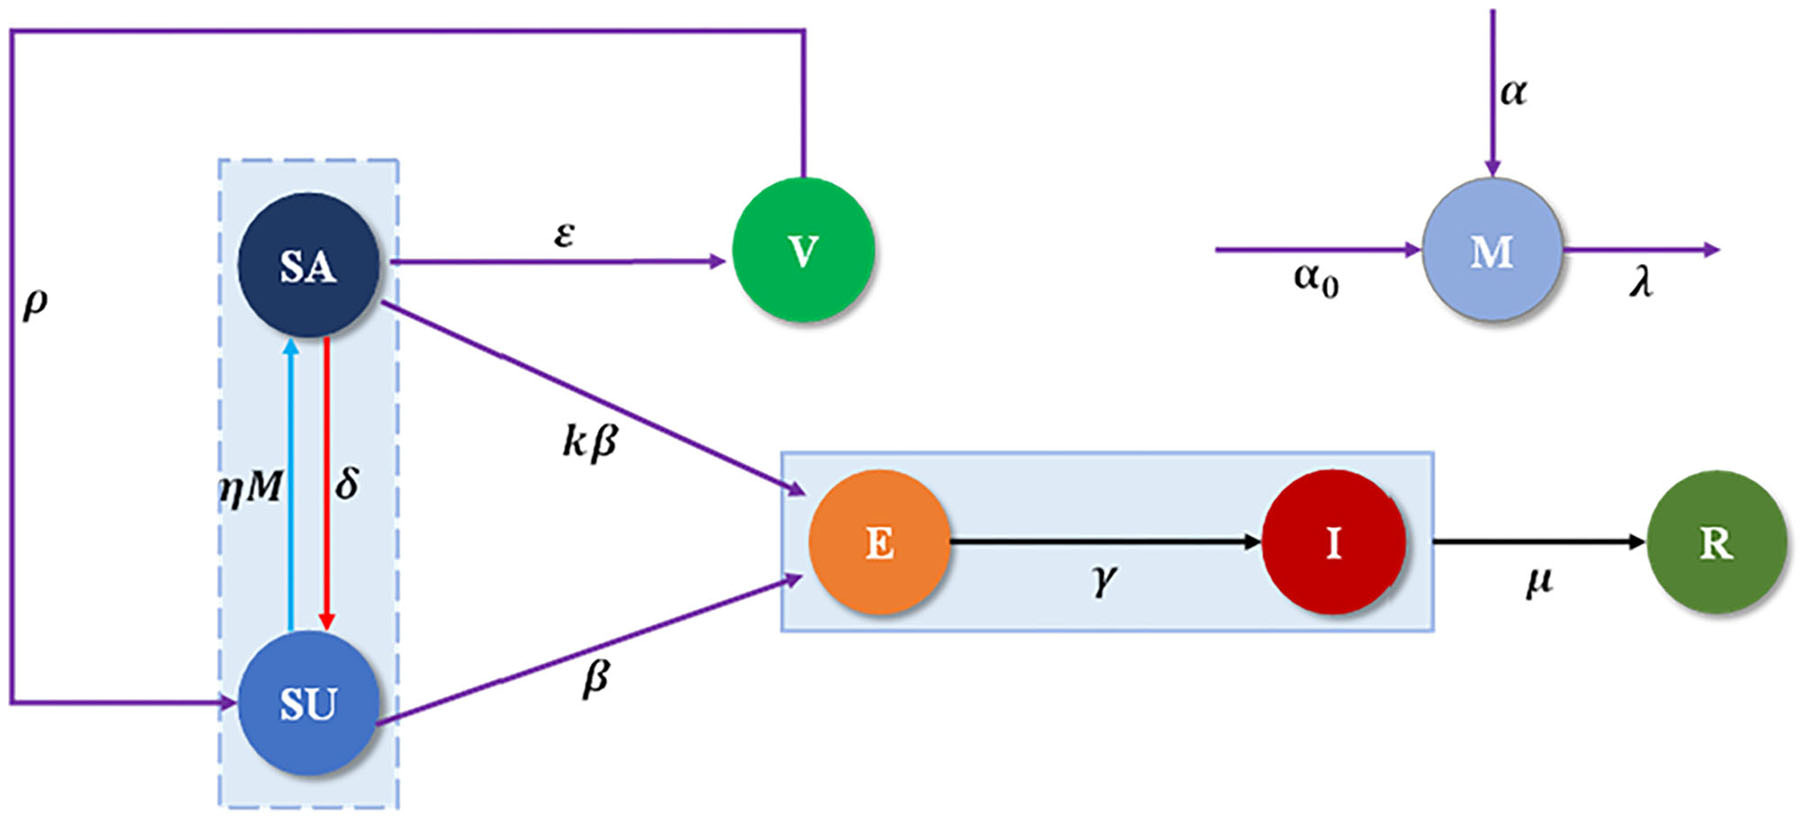
\includegraphics[width=0.6\linewidth]{0_introduction/images_review/zou_2022_SEIRVM}} \\
	\caption[Mean field models literature review]{a) The model presented in \cite{Tanaka_2002} shows horizontal layers representing behavioral diffusion, while vertical layers represent disease spread. Behavior diffuses between both infected and susceptible individuals, but this is not depicted for visual clarity. b) The model developed in \cite{Zuo2022} incorporates behavior dynamics only in the susceptible ($S$) layer, influencing both contagion rates and the probability of vaccination. The $M$ compartment, which is the accumulated density of awareness programs, follows its own dynamics, observing the state of the disease and the distribution of public opinion, and it influences the diffusion of awareness.}
	\label{fig:mean_models_1}
\end{figure}

An interesting article on the subject of behavior and vaccines is \cite{Epstein_2021}. In this model, an initially susceptible population can split into two opposing compartments, depending on what they fear more: the disease or vaccination. The model includes six compartments, with the fear dynamics occurring only in the susceptible ($S$) compartment.

In this scenario, fear of vaccination can undermine outbreak control. Initially, people may get vaccinated, but they stop too early as their fears reverse. The study also conducts a sensitivity analysis on the contact rates for the two fears, showing that transmission speed significantly affects the model’s outcomes. The results range from multiple infection waves to complete disease extinction without an outbreak, depending on the conditions.

\section{Perspective review of the literature}
To conclude this chapter on the literature review, an evaluation of the models discussed is presented, with a focus on how they relate to the scope and aim of this thesis. This evaluation wants to explain the key insights gained from the literature and highlight also what are the differences and novelty introduced in this work.

\subsection{Individual state models}
Referring to the individual-based models presented in the previous section \ref{subsec:individual_state}, most face the challenge of developing complex simulations to model the evolution of disease and individual behavior, but struggle to scale these simulations to the nationwide level. In many cases, small groups of agents are used, such as the 50 nodes mentioned in \cite{Nunner2021}, and even in works where a larger number of nodes is implemented, the count is typically in the thousands \cite{Granell2013}, not in the millions, as would be necessary for national-scale modeling. To overcome this difficulty, some articles use mean-field approximations, considering the limit of an infinite population size and employing statistical approaches \cite{Frieswijk_2022}.

Another critical issue these models face is the need for large amounts of data to accurately represent how populations behave during unusual situations like epidemic outbreaks. Without this data, it becomes difficult to draw precise conclusions from the models. While these models can still provide useful insights, their application for making precise, real-world predictions remains limited. They are better suited as scientific tools for exploring theoretical scenarios rather than for offering actionable advice on a larger scale. An article that demonstrates the volume of data required to test a model with real-world scenarios is \cite{Kemp_2021}. In this study, data from three different countries—Luxembourg, Austria, and Sweden—was collected, including information on total detected cases, hospitalized individuals, people in intensive care units (ICUs), and deaths. This comprehensive dataset was used to fit the model.

In the case of behavioral-epidemic models, even fewer data were available until the recent COVID-19 pandemic. As explained in \cite{Gosak2021}, this lack of data was a significant challenge. However, they show how it was partially addressed by implementing models based on population behavior with respect to influence. Despite these improvements, the availability of data today is certainly better, offering more robust insights. As they say: \textit{"The issue is that research has not yet provided empirical benchmarks for endogenous contact rates in disease scenarios, so it is unclear how such policies can be evaluated scientifically: ideally a policy is benchmarked against a set of counterfactuals given the disease, not compared with what was before the disease".}

\subsection{Well-mixed population models}
As stated earlier in paragraph \ref{subsec:homogeneous}, a major critique of developing complex mean-field models is that if they are not supported by consistent observation of the phenomena they aim to reproduce, their capacity to generate meaningful insights can be significantly limited. For this reason, confront and develop a model using empirical data as reference, is one of the main objectives pursued in this thesis work. The comparison of the model's emerging dynamics with real-world data is a reliable method to test the model's validity and evaluate its predictive capacity.
Reading through works in this field, a common approach emerges for modeling systems that aim to incorporate two distinct dynamics, such as behavior and disease spread. Most of these models introduce additional compartments, which represent subgroups of homogeneously mixed individuals sharing common characteristics—typically, their disease state and course of action. The primary distinction lies in how modelers handle the flow between these compartments: while some works focus on the influence of behavior solely within the Susceptible layer \cite{Epstein_2021, Tyson_2020, Zuo2022}, others implement a full double-layer model \cite{Bongarti2023, Bulai2023, Tanaka_2002}. Another key difference is whether the change in behavior dynamics is unidirectional, as in \cite{Bongarti2023}, or bidirectional, as seen in \cite{Epstein_2021, Tyson_2020, Tanaka_2002, Zuo2022}, where individuals can adjust their actions in both directions.
Notably, some of the most influential aspects drawn from the literature for this thesis include the "double fear" structure developed by \cite{Epstein_2021} and the awareness element that influences behavior change, modeled through an external node $M(t)$ in \cite{Zuo2022}. Additionally, this thesis seeks to implement a fully coupled double-layer model for behavior and epidemic spread, incorporating elements such as memory waning and fatigue, which combine with conversational mechanisms to create bidirectional flows in the behavioral model.
Unlike \cite{Tanaka_2002}, which uses a simpler epidemic model, this work employs a more complex one to accurately reflect COVID-19 data. Furthermore, the models developed in \cite{Bulai2023} and \cite{Smaldino_2021} share structural similarities with this thesis. However, \cite{Bulai2023} assumes faster information diffusion than disease transmission, decoupling the two layers, while \cite{Smaldino_2021} focuses on homophily and polarization of compartments—factors not considered here due to data limitations.

\subsection{Final remarks}
All the concepts presented in this chapter are useful for understanding the current state of epidemic behavior modeling and for explaining why the development of a new model was necessary for this thesis.

To summarize, the main features sought in a model are:

\begin{itemize} 
	\item Comparability to empirical data collected during a real epidemic, both for the disease and the behavioral layer. 
	\item In a mean-field system, the ability to model disease incidence, peer pressure between individuals with different behaviors, fatigue in maintaining certain habits, and the possibility to modify this dynamic by introducing a mean-field intervention, such as government actions, to encourage the transition to more compliant behavior. 
	\item Avoidance of using awareness as a factor in the model, as it is too abstract and difficult to observe or measure within a population; instead, focusing on behavior dynamics and peer-to-peer imitation based on which behavior appears most convincing. 
	\item Exclusion of vaccination dynamics, as it is a well-known aspect and, in the case of COVID-19, vaccines were only available on a large scale after more than a year. 
\end{itemize}

All these characteristics have been incorporated, and the following chapter will explain how the model was developed and how these features were integrated.
